We tested and verified our algorithm using two examples of different difficulty.
The first example is a small polypeptide alpha-conotoxin
PnIB. We generated the EDM for this example from the coordinates of
the polypeptide. The second example is the fitting the GroEL domains
into the electron density map of the GroEL complex.

\subsection{Alpha-conotoxin PnIB}
First, we explored the relationship between encoding quality and the quality of the fitting. For this purpose, we chose the small 16--residue polypeptide alpha-conotoxin
PnIB. We downloaded the X-ray crystal structure of alpha-conotoxin PnIB (PDB code
1AKG) \cite{Guimond2009} from the PDB database \cite{Berman2000} and
simulated the electron density map (2mFo-DFc) using the Uppsala electron density server \cite{Kleywegt2004} with the resolution $R=1.1$ \AA.
We computed the protein density according to  Eq. \ref{eq:protein_density}
with the Gaussian width $\alpha=1.0$ \AA~ using
only the non-hydrogen atoms of the standard amino acids. We rotated the initial 1AKG structure by the arbitrarily chosen Euler angles equal to 
76, 234, and 56 degrees, respectively, and used it as the input for the fitting workflow.
We used $N_{rot}=500$ (corresponding to an angular step of 36\textdegree ) rotations represented with uniformly 
distributed Euler angles spanning the space of $2\pi\times\pi\times 2\pi$. 
The order of the Hermite expansion
was set to $N=15$, which is the minimum expansion order allowed at this resolution according to Eq. \ref{eq:Nmin}. 
The order of the Fourier expansion was twice the order of the Hermite expansion, $M=30$ for each dimension.

To see how the encoding quality influences the fitting algorithm, we studied the dependence of the decomposition on the scaling
parameter $\lambda$. We chose a range of $\lambda$ parameters between
0.05 and 2.0. For each $\lambda$, we computed the best fitting score along with the average fitting score. 
Fitting results are shown in Fig. \ref{fig:test1AKG}.
We see that by choosing $\lambda$ small,
we neglect the details of the protein structure (Fig. \ref{fig:test1AKG} A) and therefore, we can not discriminate between different orientations
of the protein (maximum score for $\lambda=0.05$ is very close to
the average score). When choosing $\lambda$ sufficiently large, we
obtain satisfactory discriminative power to find the near-native position
of the protein (Fig. \ref{fig:test1AKG} C,D). We also see that,
e.g., for $\lambda=0.5$, the difference between the maximum and the
average score is much larger than in the case of $\lambda=0.05$.
Also, when we take $\lambda$ too large, we can not encode the whole
protein (Fig. \ref{fig:test1AKG} E). 
%
The red dashed line on Fig. \ref{fig:test1AKG} shows R-factors computed with Eq. \ref{eq:Rfactor}.
We see that the choice of parameter $\lambda$ influences the R-factors and thus determines the quality of the fitting. 
Notably, the minimum of the R-factor curve corresponds to the maximum
of the fitting score.


Due to the strong influence of the scaling parameter $\lambda$ on the discrimination power of the algorithm,
we estimated its optimal value to gain the maximum separation between the score of the correct pose and the average score. 
%
Provided that the box that contains all the rotations of the peptide has the size $L_{box}=23$~\AA~and setting the resolution of the 
EDM $R=1.1$ {\AA}, Eq. \ref{eq:LambdaEstimate} gives an estimate on the optimal value of the scaling parameter $\lambda_{opt}\approx0.50$.
%
Fig. \ref{fig:test1AKG} shows
that this estimation corresponds to the best discrimination
between the near-native and all other structures, which can be deduced
from the maximum separation between the score of the prediction and
the average score. 
RMSD between the prediction and the solution at this value of $\lambda$ is $1.03$ \AA .
%
We should note that the RMSD can be  decreased by taking a finer angular search step.


\begin{figure}[h]
\label{fig:test1AKG}
\begin{centering}
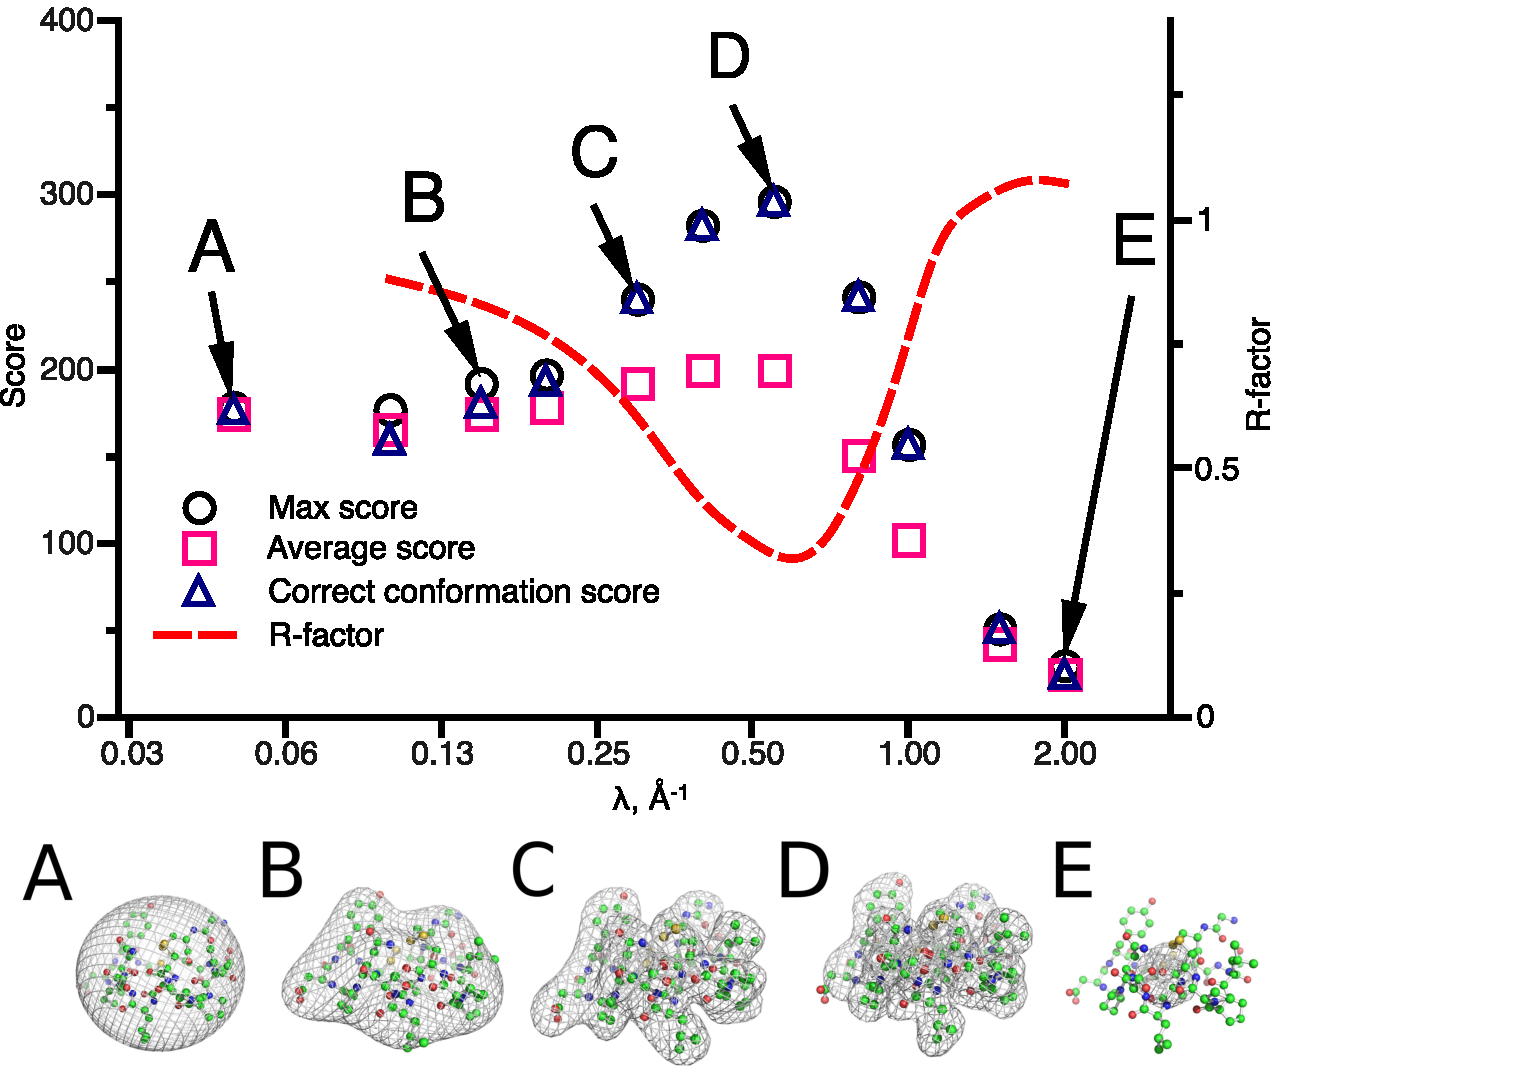
\includegraphics[width=1\textwidth]{Hermite/Fig/ScoreDescriminationVsLambdaAndRFactor-rev.pdf}
\par\end{centering}
\caption[Results for the alpha-conotoxin PnIB]{Test of the fitting algorithm on artificially generated EDM for the alpha-conotoxin PnIB (PDB code 1AKG).
Here, we plotted the dependence of four parameters, the maximum score, the average score, the score of the near-native conformation and the crystallographic R-factor on the scaling
parameter $\lambda$. 
Isosurface of the Hermite decomposition at protein model density equal to $ (\rho_{max}+\rho_{min})/2 $ and several values of $\lambda$ are shown in sub-plots A ($\lambda=0.05$),
B ($\lambda=0.15$), C ($\lambda=0.3$), D ($\lambda=0.55$) and E ($\lambda=2.0$). }
\end{figure}

\subsection{GroEL complex}
Here, we demonstrate that our approach obtains essentially the same results as other programs, provided that the scoring function if the same (LCCF in this case).
For this purpose, we use a classical test for a fitting algorithm, the GroEL complex map. 
We downloaded the EDM of the GroEL complex from the Electron Microscopy Data Bank (EMDB), code EMD-2001 with 
resolution of 8.5~\AA.
Then, we downloaded the crystal structure of the GroEL subunits from the PDB database. We used the GroEL-GroES complex (PDB code 1AON), from which we extracted the chain A, 
centered it and arbitrary rotated to exclude any bias.
We chose the sampling grid size according to the resolution and the size of the EDM. The EDM was first padded with zeros and then transformed to the Fourier basis using the FFT algorithm.
The number of coefficients in the Fourier decomposition $M$
was equal to $ 105 \times 107 \times 119 $.
The angular search step was set to 30\textdegree. 
We used the Hermite expansion order of $N=15$, which is larger than the minimum expansion order allowed at this resolution, $N_{min}\approx9$ (see Eq. \ref{eq:Nmin}).
We sampled the rotations using the spiral algorithm \cite{saff1997distributing},
which generates an equispaced distribution of points on a sphere.
Unlike in the previous example, due to the lower resolution of the GroEL EDM, here we fitted Laplacian filtered protein density into the Laplacian filtered EDM.

After the 6D exhaustive search, we clustered the solutions using the clustering threshold of 10~\AA~ and kept the top 14 poses.
All the 14 poses corresponded to the individual chains of the complex, which comprises 2 heptameric rings structure.
Fig. \ref{fig:GroEL_FIT} shows the result of the fitting. 
We compared the fitted model with the model provided by the authors of the EDM (PDB entry code 4AAU). The average RMSD between the chains due to flexible deformations measured using C$\alpha$ atoms 
was 3.0~\AA.
More precisely,
we super-posed the corresponding chains of both models using rigid-body transformations and then measured RMSD between them. 
%
Overall, the average RMSD between C$\alpha$ atoms was 5.35~\AA.
This includes both the discrepancy between corresponding chains in the assembly due to flexible deformations and because of the rigid body misfit. 
The average distance between the centers of mass of the corresponding chains was 2.64~\AA~(Table \ref{table:RMSDComparisson}).

\begin{table}[h]
\begin{centering}
\begin{tabular}{|c|c|c|}
\hline
Algorithm & RMSD $C_{\alpha}$, ~\AA & RMSD centers of masses, ~\AA \\ \hline 
ADP\underline{\hspace*{0.2cm}}EM & 4.61 & 2.29  \\ \hline 
Colores & 5.42 & 2.52  \\ \hline 
HermiteFit & 5.35 & 2.64 \\ \hline 
\end{tabular}
\medskip
\caption[Comparison of the models obtained using HermiteFit, Colores and ADP\underline{\hspace*{0.2cm}}EM algorithms by RMSD]{ 
Comparison of the models obtained using HermiteFit, Colores and ADP\underline{\hspace*{0.2cm}}EM algorithms with the model obtained by the authors of the electron density map (PDB entry 4AAU).
For each pair of models, RMSD was measured using the $C_{\alpha}$-atoms and the centers of mass of the corresponding chains and then averaged over all chains comprising the assembly.}
\label{table:RMSDComparisson}
\par\end{centering}
\end{table}


\begin{figure}[h]
\label{fig:GroEL_FIT}
\begin{centering}
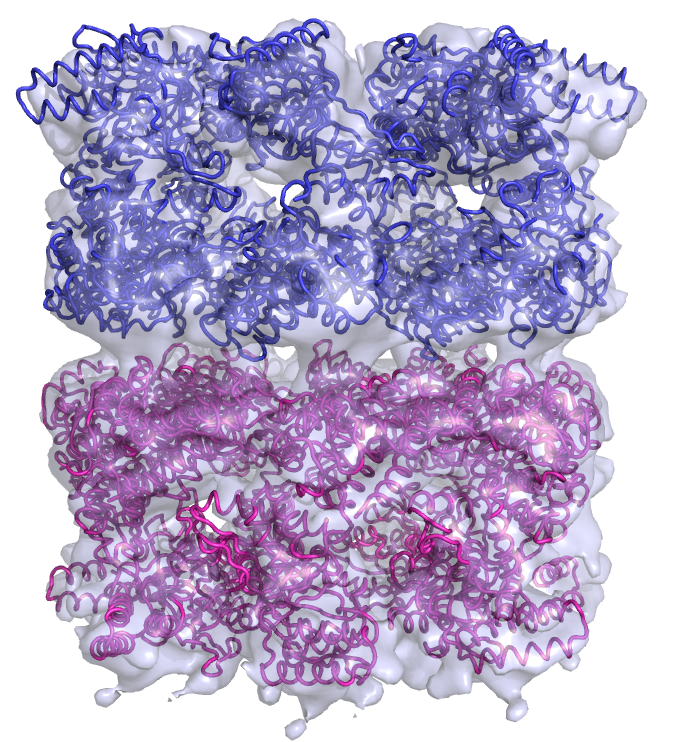
\includegraphics[width=0.5\textwidth]{Hermite/Fig/figure8}
\par\end{centering}
\caption[Result of the fitting of the GroEL EDM]{Result of the fitting chain A of the GroEL-GroES X-Ray structure (PDB entry 1AON) to the GroEL complex electron density map (EMD-2001). 
Two heptameric rings are shown in different colors. The average RMSD  measured using the $C_{\alpha}$-atoms between the two closest chains in the fitted structure and the flexibly refined structure provided by the authors
of the EDM (PDB entry 4AAU) is 5.35~\AA} .
\end{figure}

\subsection{Runtime of Hermite- to Fourier- space transition}
The use of the fast Fourier transform was the inevitable step in every fitting algorithm up until now. 
Instead, we introduced the basis from which we can 
transform a decomposition into the Fourier basis avoiding evaluation of the FFT on a grid. 
When the grid becomes large, %($M\rightarrow \infty$), 
the asymptotic complexity of our algorithm becomes $O\left( M^3 N \right)$ (see Eq. \ref{eq:HermiteFourierSum}
). It is comparable to the complexity of the fast Fourier transform 
algorithm, $O\left( M^3 \log M   \right)$. 
Intuitively, at large orders of the Fourier expansion $M$, our algorithm should be faster compared to the FFT. 
However, prefactors preceded the complexities of the two algorithms are different. Thus, we conducted 
a numerical experiment to compare the actual running times. 
Fig. \ref{fig:Hermite_FFT_speed} shows the time needed to compute the FFT on a cubic grid of size $M$ and the 
time needed to transform a Hermite expansion of order $N=15$ to the same Fourier grid. 
%
We can see that, generally, at large values of $M$, $M\gtrapprox 100$, the transition from the Hermite into the Fourier space is faster compared to the speed of the FFT. 
Also, the timing of the transition grows evenly with respect to $M$ in contrast to the timing of the FFT.
%
One has to take into account that we compared our algorithm with the highly optimized FFTW3 library \cite{frigo2005design}. 
Probably, additional optimization of HermiteFit could improve performance even further. One of the ways to speed up the transition 
will be to use the Fast Hermite Transform instead of the naive matrix multiplication \cite{leibon2008fast}. This implementation will be the subject of our future work.

\begin{figure}[h]
\label{fig:Hermite_FFT_speed}
\begin{centering}
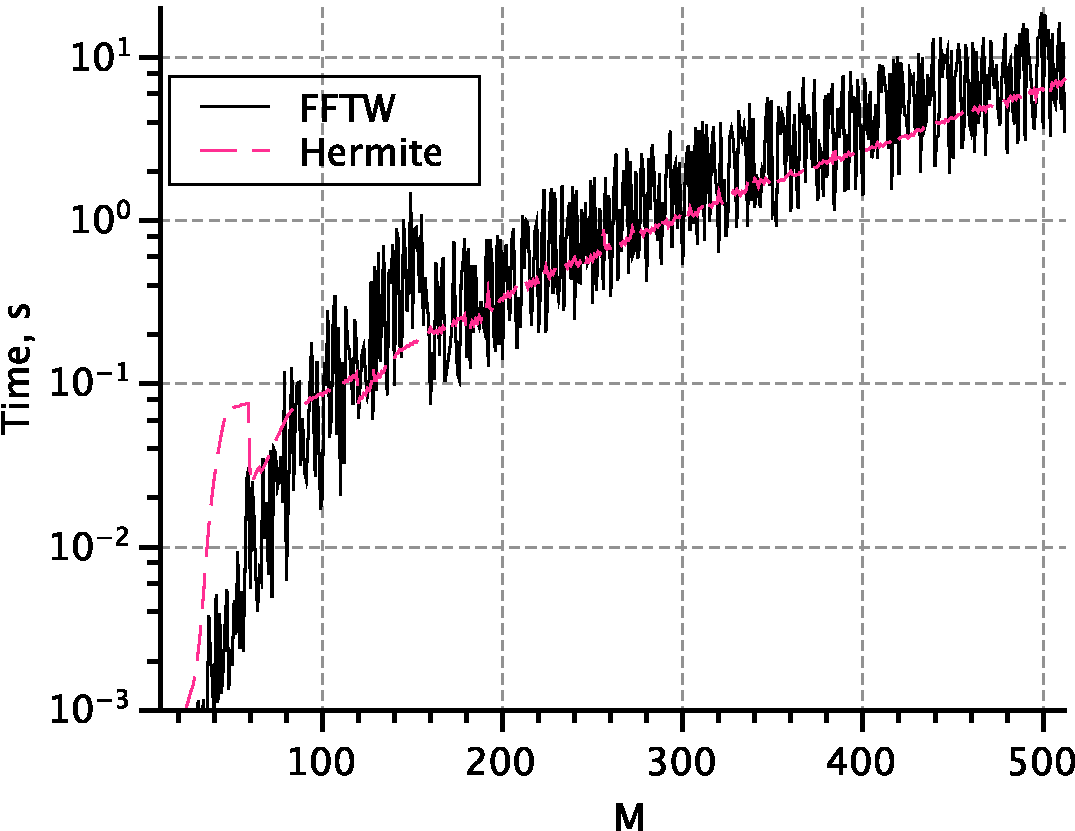
\includegraphics[width=0.5\textwidth]{Hermite/Fig/figure9.pdf}
\par\end{centering}
\caption[Running times of the Hermite to Fourier space transition and FFTW]{Running times of the Hermite to Fourier space transition performed using our algorithm and the FFT algorithm on a cubic grid of $M\times M\times M$ as a function of the Fourier expansion order $M$.
We used the FFTW3 library \cite{frigo2005design} with the double precision real discrete Fourier transform using the flag FFTW\_ESTIMATE to measure the speed of the FFT. The order of the Hermite expansion was $N=15$.}
\end{figure}

\subsection{Comparison with Situs and ADP\underline{\hspace*{0.2cm}}EM}
We compared the HermiteFit algorithm with two popular existing fitting methods, the {\em colores} program
from the Situs package \cite{Chacon2002} and the ADP\underline{\hspace*{0.2cm}}EM fitting tool  \cite{garzon2007adp_em}. 
These two packages represent the two major approaches to the problem of exhaustive search in the six-dimensional space of rigid-body motions.
{\em Colores}, a widely used 
CCF-based fitting tool, rapidly scans the translational degrees of freedom using the fast Fourier transform.  The rotations, though, are sampled exhaustively 
by enumerating a list of equispaced distributed rotations on a sphere.
ADP\underline{\hspace*{0.2cm}}EM 
choses points in real space, places there the atomic structure and then rotationally matches it to the EDM using the Fast Rotational Matching algorithm.
The authors of the ADP\underline{\hspace*{0.2cm}}EM compared their algorithm with the 5D rotational matching and found that the 3D rotational matching works faster 
in practice \cite{garzon2007adp_em}. 

For the comparison, we normalized the running time of the fitting algorithms by the sizes of the search space. 
For {\em colores} and HermiteFit, the size of the search space is equal to the number of grid cells ($M^3$ for a cubic grid in the HermiteFit algorithm) multiplied by the number of sampled angles.
The size of the search space of the ADP\underline{\hspace*{0.2cm}}EM algorithm is the number of points in real space times the number of cells of the angular grid. The latter is
built from uniformly sampled Euler angles on a grid of $2\pi\times\pi\times 2\pi$. The size of the angular grid is determined by the order $N_{exp}$ of 
a spherical harmonics expansion and equals to $4N_{exp}^3$.
For {\em colores} and HermiteFit, we used the angular search step of 30\textdegree. The resolution of the EDM 
for {\em colores} and HermiteFit was set to 8.5~\AA. The Fourier grid that was used by {\em colores} and the HermiteFit algorithm had dimensions $105 \times 107 \times 119$.
For ADP\underline{\hspace*{0.2cm}}EM, we used the spherical harmonics expansion order of $N_{exp}=16$.


Table \ref{table:PerPointEffectiveness} shows the normalized times of the complete 6D search for the three algorithms in the case of fitting the GroEL subunit into 
the 8.5~\AA~GroEL electron density map. 
%
Judging by the total running time, ADP\underline{\hspace*{0.2cm}}EM has a big advantage over the two other algorithms, which exhaustively search all the space of possible translations. 
However,
in terms of running time per one search point, the HermiteFit algorithm is more effective than the other two.
%
Interestingly, {\em colores}  spends about half of the total search time on the computation of the Fourier coefficients of the rotated protein. Therefore, it was very important for us to speed up this step. 
Nonetheless, all three tested algorithms have their own advantages and drawbacks. For example, ADP\underline{\hspace*{0.2cm}}EM can use smart heuristics to contract the number of
search points in the real space. However, its sample points in the space of rigid body rotations are distributed non-uniformly.
In particular, near the poles rotations are sampled more densely, making this sampling scheme less effective \cite{saff1997distributing}. 
On the other hand, the HermiteFit algorithm along with the {\em colores} algorithm sample the rotational space nearly uniformly using the spiral algorithm
while the translational space sampling also remains uniform. 
%
We would like to stress that the absolute runtimes (shown in Table \ref{table:PerPointEffectiveness}) are not very informative. In particular, they dramatically depend on the choice of the FFT library, code optimization, the choice of compiler and compilation options, etc. However, this comparison clearly demonstrates that the new approach paves the way to speed up one of the bottlenecks of fitting methods, the projection of the rotated structure into the Fourier space.

%
To assess the fitting quality of the tested methods, we measured the RMSDs between the obtained models and the structure obtained by the authors of 
the electron density map (PDB entry 4AAU). 
Table \ref{table:RMSDComparisson} shows the comparison of the measured RMSDs for ADP\underline{\hspace*{0.2cm}}EM, {\em colores} and HermiteFit.
We used two different criteria for the measurements. 
First, we  measured the average RMSD between $\alpha$-carbons. Second, we measured the average distance between the centers of mass of the corresponding chains.
%
 ADP\underline{\hspace*{0.2cm}}EM produced a model with RMSD of $4.61$ \AA~ from the solution, RMSDs for {\em colores} and HermiteFit were $5.42$ \AA~ and $5.35$ \AA, respectively.
%
Clearly, Table \ref{table:RMSDComparisson} demonstrates that the tested algorithms produce equal quality models.
However, results of ADP\underline{\hspace*{0.2cm}}EM are slightly better, presumably because of the finer rotational sampling.

\begin{table}[h]\small
\begin{centering}
\resizebox{\textwidth}{!} {
\begin{tabular}{|c|c|c|c|c|}
\hline
Algorithm & Num of rot-space points & Num of trans-space points & Runtime, s & Time per point, $\times 10^{-7}$s \\ \hline 
ADP\underline{\hspace*{0.2cm}}EM & 16384 & 23186 & 139 & 3.6 \\ \hline 
Colores & 4416 & 1336965 & 1454 & 2.5  \\ \hline 
HermiteFit & 4416 & 1336965 & 917 & 1.5  \\ \hline 
\end{tabular}
}
\medskip
\caption[Comparison of the HermiteFit algorithm with the Colores and ADP\underline{\hspace*{0.2cm}}EM algorithms by runtime]{ Comparison of the HermiteFit algorithm with the Colores and ADP\underline{\hspace*{0.2cm}}EM algorithms. The comparison criterion was chosen to be
the total running time and the running time per one point of the search space.}
\label{table:PerPointEffectiveness}
\par\end{centering}
\end{table}
